\chapter{Preliminares}

Tras una breve introducción a los dispositivos que se usarán para el desarrollo de esta obra, procederemos a las primeros pasos necesarios para la configuración y control de los drones.

En adelante, se detallan los procedimientos para lo que es conocido como \textit{Maiden Flight}, 
el primer vuelo de cualquier tipo de vehículo aeronáutico o aeroespacial. 
Posteriormente, tras las pruebas con el firmware y software oficiales, se realizarán las mismas pruebas con el firmware del proyecto Paparazzi UAV.

%%%%%%%%%%%%%%%%%%%%%%%%%%%%%%%%%%%%%%%%%%%%%%%%%%%%%%%%%%%%%%%%%%%%%%%%%%%%%%%%%%%%%%%%%%%%%%%%%%%%%%%%%%%%%%%%%
%%%%%%%%%%%%%%%%%%%%%%%%%%%%%%%%%%%%%%%%%%%%%%%%%%%%%%%%%%%%%%%%%%%%%%%%%%%%%%%%%%%%%%%%%%%%%%%%%%%%%%%%%%%%%%%%%
%%%%%%%%%%%%%%%%%%%%%%%%%%%%%%%%%%%%%%%%%%%%%%%%%%%%%%%%%%%%%%%%%%%%%%%%%%%%%%%%%%%%%%%%%%%%%%%%%%%%%%%%%%%%%%%%%

\section{Montaje de los drones}

Cada Crazyflie 2.1 necesita de montaje manual. Para ello, se ha seguido la guía oficial del fabricante \cite{crazyflie_assembly_and_quickstart}.
Los componentes de un Crazyflie necesarios para el montaje son los siguientes:

\begin{table}[h]
\centering
\begin{tabular}{l|c}
    \multicolumn{1}{c|}{\textbf{Componente}} & \textbf{Cantidad} \\ \hline
    Crazyflie 2.1 Board             & 1        \\
    Hélices tipo CW                 & 2        \\
    Hélices tipo CCW                & 2        \\
    Anclajes para motores           & 4        \\
    Motores DC                      & 4        \\
    Batería LiPo                    & 1        \\
    Anclaje para batería            & 1        \\
    Pines de expansión              & 1       
\end{tabular}
    \caption{Componentes de un Crazyflie 2.1}
    \label{tab:componentes_crazyflie}
\end{table}

Además, podemos ver en esta figura los componentes de un Crazyflie previo a su montaje:

\begin{figure}[h]
    \centering
    \includegraphics[width=0.88\textwidth]{img/fig/fig2.1-crazyflie-disassembled.jpg}
    \caption{Componentes de un Crazyflie 2.1}
    \label{fig:crazyflie_disassembled}
\end{figure}

El procedimiento de montaje, a efectos simplificados, es el siguiente. Se sigue, como bien se ha indicado previamente, 
la guía oficial \cite{crazyflie_assembly_and_quickstart}:

\begin{itemize}
    \item Montaje de los motores en cada anclaje para estos.
    \item Insertar los anclajes en el Crazyflie 2.1 y conectar los motores eléctricamente a este.
    \item Añadir las hélices a los motores, diferenciando las CW (\textit{ClockWise}) de las CCW (\textit{CounterClockWise}).
    \item Montar los pines de expansión y la batería.
    \item Anclar la batería utilizando el anclaje de la batería, que se conecta a los pines de expansión.
\end{itemize}

%%%%%%%%%%%%%%%%%%%%%%%%%%%%%%%%%%%%%%%%%%%%%%%%%%%%%%%%%%%%%%%%%%%%%%%%%%%%%%%%%%%%%%%%%%%%%%%%%%%%%%%%%%%%%%%%%
%%%%%%%%%%%%%%%%%%%%%%%%%%%%%%%%%%%%%%%%%%%%%%%%%%%%%%%%%%%%%%%%%%%%%%%%%%%%%%%%%%%%%%%%%%%%%%%%%%%%%%%%%%%%%%%%%
%%%%%%%%%%%%%%%%%%%%%%%%%%%%%%%%%%%%%%%%%%%%%%%%%%%%%%%%%%%%%%%%%%%%%%%%%%%%%%%%%%%%%%%%%%%%%%%%%%%%%%%%%%%%%%%%%

\section{Pruebas con software oficial}

Con un Crazyflie montado, podemos proceder a las pruebas iniciales con el conjunto de software y firmware oficial.
Desde la guía oficial de montaje se recomienda utilizar la máquina virtual preconfigurada por Bitcraze para conseguir
volar el rotorcraft lo antes posible \cite{bitcraze_vm}. En esta máquina virtual se incluye los programas para el control,
código fuente y otros recursos software de utilidad para el desarrollo con Crazyflies.

%%%%%%%%%%%%%%%%%%%%%%%%%%%%%%%%%%%%%%%%%%%%%%%%%%%%%%%%%%%%%%%%%%%%%%%%%%%%%%%%%%%%%%%%%%%%%%%%%%%%%%%%%%%%%%%%%
%%%%%%%%%%%%%%%%%%%%%%%%%%%%%%%%%%%%%%%%%%%%%%%%%%%%%%%%%%%%%%%%%%%%%%%%%%%%%%%%%%%%%%%%%%%%%%%%%%%%%%%%%%%%%%%%%
%%%%%%%%%%%%%%%%%%%%%%%%%%%%%%%%%%%%%%%%%%%%%%%%%%%%%%%%%%%%%%%%%%%%%%%%%%%%%%%%%%%%%%%%%%%%%%%%%%%%%%%%%%%%%%%%%

\subsection{Preparación}

Previo a la conexión con un Crazyflie, debemos de cargar el firmware al Crazyradio 2.0, el módulo USB que nos permite controlar 
remotamente un Crazyflie y recibir telemetría de este. Para ello, se sigue la guía oficial del fabricante \cite{crazyradio_setup}.

\begin{figure}[h]
    \centering
    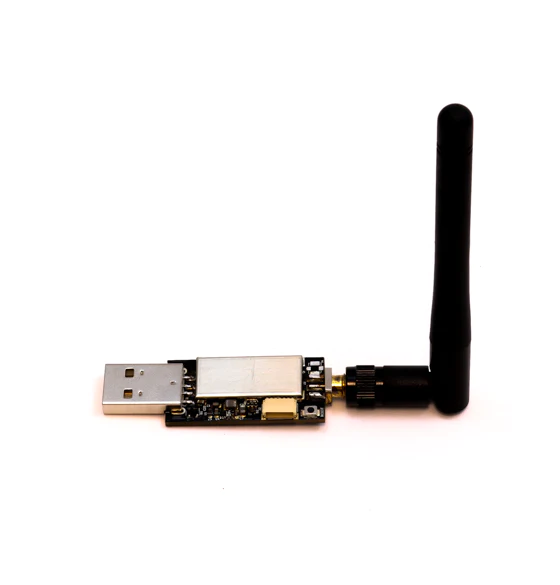
\includegraphics[width=0.65\textwidth]{img/fig/fig2.2-crazyradio.png}
    \caption{Crazyradio 2.0}
    \label{fig:crazyradio}
\end{figure}

Con ello, ya podemos conectarnos a un Crazyflie desde el software de control Crazyflie Client, no obstante, 
se recomienda actualizar el firmware del Crazyflie 2.1 previamente utilizando Crazyflie Client. 
Se sigue la guía oficial de actualización de firmware \cite{crazyflie_firmware_upgrade}.

%%%%%%%%%%%%%%%%%%%%%%%%%%%%%%%%%%%%%%%%%%%%%%%%%%%%%%%%%%%%%%%%%%%%%%%%%%%%%%%%%%%%%%%%%%%%%%%%%%%%%%%%%%%%%%%%%
%%%%%%%%%%%%%%%%%%%%%%%%%%%%%%%%%%%%%%%%%%%%%%%%%%%%%%%%%%%%%%%%%%%%%%%%%%%%%%%%%%%%%%%%%%%%%%%%%%%%%%%%%%%%%%%%%
%%%%%%%%%%%%%%%%%%%%%%%%%%%%%%%%%%%%%%%%%%%%%%%%%%%%%%%%%%%%%%%%%%%%%%%%%%%%%%%%%%%%%%%%%%%%%%%%%%%%%%%%%%%%%%%%%

\subsection{Control básico con Crazyflie Client}

El último paso previo a cambiar al proyecto Paparazzi consiste en familiarizarse con el control básico de un solo Crazyflie 
mediante el software oficial. De esta forma se confirma también el correcto funcionamiento de cada dron, asegurando que no es fallo
de firmware/software no oficiales (Paparazzi, en este caso). Aquí podemos ver la interfaz de Crazyflie Client:

\begin{figure}[h]
    \centering
    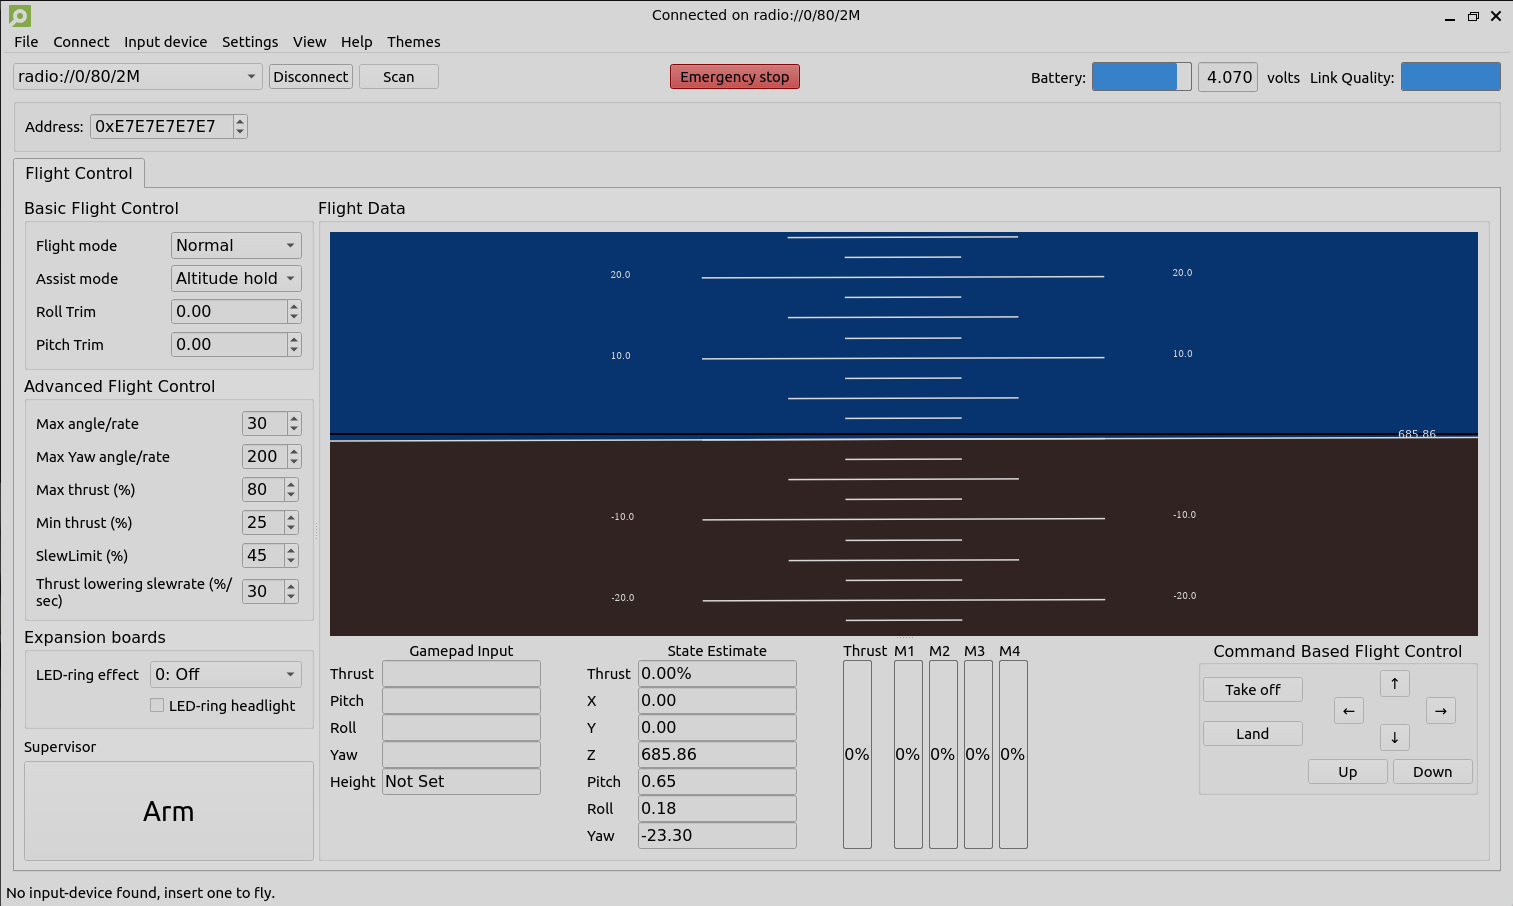
\includegraphics[width=0.96\textwidth]{img/fig/fig2.3-crazyflie-client.png}
    \caption{Interfaz de Crazyflie Client}
    \label{fig:crazyflie-client}
\end{figure}

\subsection{Variables de control en Crazyflie Client}

Previo a continuar con el desarrollo de este trabajo, es importante entender las variables básicas que definen como se desarrolla el vuelo de un rotorcraft.
Aunque existen más, introduciremos aquí todas las variables que Crazyflie Client nos permite saber de un Crazyflie. 

En la siguiente tabla se detallan las variables, así como la unidad del Sistema Internacional que se utiliza. 
Se indican unidades alternativas entre paréntesis, muy utilizadas en otras situaciones o programas. 

\begin{table}[h]
\centering
\begin{tabular}{c|c|c}
    \textbf{Variable} & \textbf{Descripción} & \textbf{Unidad} \\ \hline
    Roll     & Rotación sobre el eje X   & Grados (Radianes) \\
    Pitch    & Rotación sobre el eje Y   & Grados (Radianes) \\
    Yaw      & Rotación sobre el eje Z   & Grados (Radianes) \\
    X        & Posición en el eje X      & m                 \\
    Y        & Posición en el eje Y      & m                 \\
    Z        & Posición en el eje Z      & m                 \\
    Height   & Altura respecto al suelo  & m                 \\
    Thrust   & Empuje de los motores     & \%                \\
    Battery  & Nivel restante de batería & V (\%)            
\end{tabular}
    \caption{Variables de control de un Crazyflie en Crazyflie Client}
    \label{tab:crazyflie_client_vars}
\end{table}

Cabe destacar las variables \textbf{roll, pitch y yaw} que indican la rotación de un objeto respecto a alguno de sus ejes.
Son variables muy usadas en el ámbito de control de vehículos aéreos y aeroespaciales. La siguiente imagen describe de forma 
gráfica cada una de estas variables.

\begin{figure}[h]
    \centering
    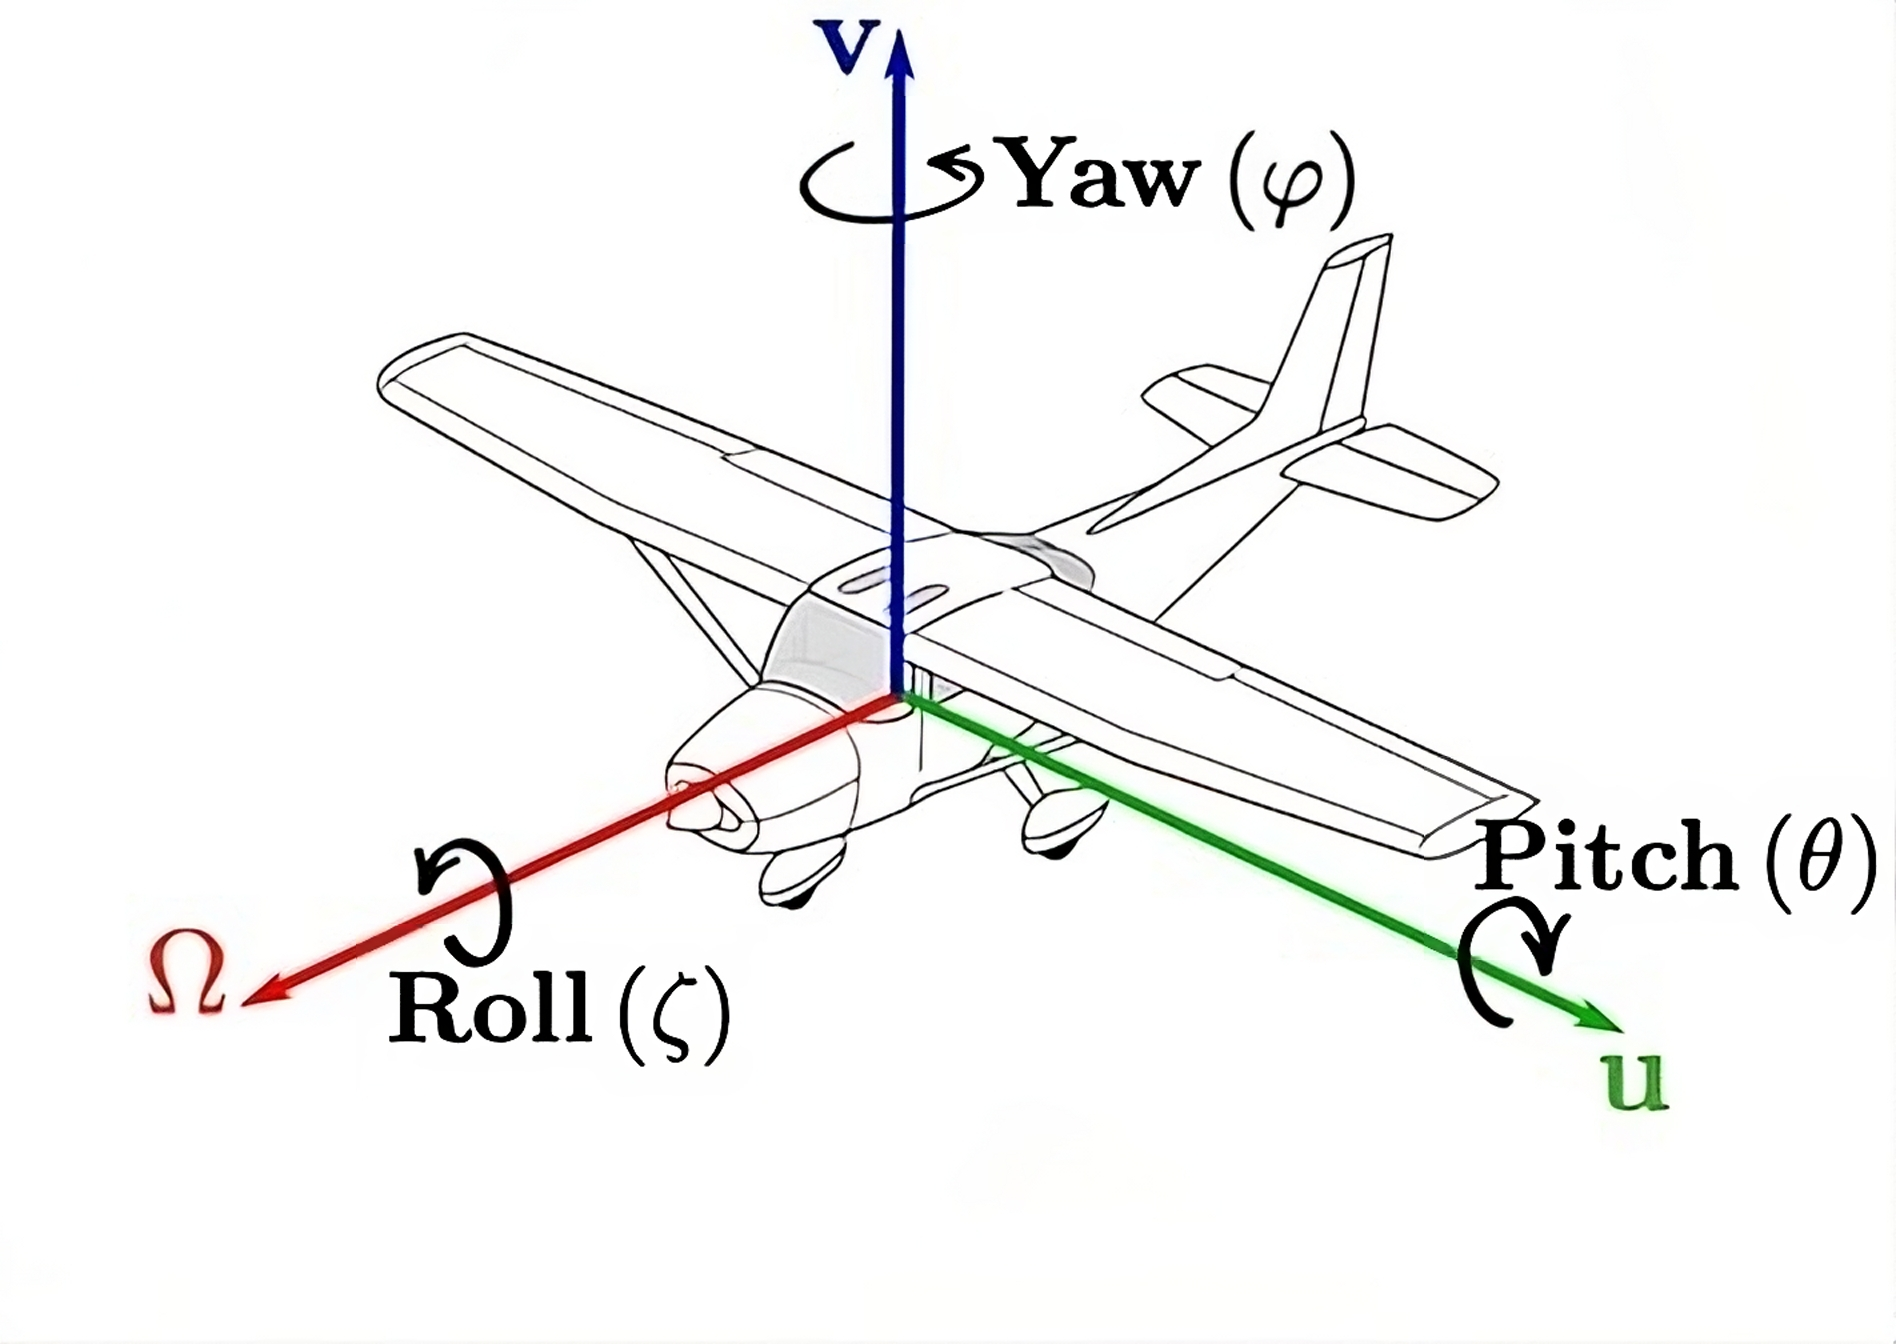
\includegraphics[width=0.9\textwidth]{img/fig/fig2.4-rotational-axes.jpeg}
    \caption{Ejes de rotación de un vehículo aéreo}
    \label{fig:rotational-axes}
\end{figure}

%%%%%%%%%%%%%%%%%%%%%%%%%%%%%%%%%%%%%%%%%%%%%%%%%%%%%%%%%%%%%%%%%%%%%%%%%%%%%%%%%%%%%%%%%%%%%%%%%%%%%%%%%%%%%%%%%
%%%%%%%%%%%%%%%%%%%%%%%%%%%%%%%%%%%%%%%%%%%%%%%%%%%%%%%%%%%%%%%%%%%%%%%%%%%%%%%%%%%%%%%%%%%%%%%%%%%%%%%%%%%%%%%%%
%%%%%%%%%%%%%%%%%%%%%%%%%%%%%%%%%%%%%%%%%%%%%%%%%%%%%%%%%%%%%%%%%%%%%%%%%%%%%%%%%%%%%%%%%%%%%%%%%%%%%%%%%%%%%%%%%

\section{Pruebas con Paparazzi UAV}

Realizadas el montaje y pruebas iniciales, el siguiente paso consiste en la familiarización con el ecosistema Paparazzi.
Se instalará Paparazzi Center y acto seguido se realizará una breve simulación de vuelo en Paparazzi GCS. 
Tras ello, se cargará el firmware de Paparazzi para un Crazyflie y se realizará la primera prueba real.

%%%%%%%%%%%%%%%%%%%%%%%%%%%%%%%%%%%%%%%%%%%%%%%%%%%%%%%%%%%%%%%%%%%%%%%%%%%%%%%%%%%%%%%%%%%%%%%%%%%%%%%%%%%%%%%%%
%%%%%%%%%%%%%%%%%%%%%%%%%%%%%%%%%%%%%%%%%%%%%%%%%%%%%%%%%%%%%%%%%%%%%%%%%%%%%%%%%%%%%%%%%%%%%%%%%%%%%%%%%%%%%%%%%
%%%%%%%%%%%%%%%%%%%%%%%%%%%%%%%%%%%%%%%%%%%%%%%%%%%%%%%%%%%%%%%%%%%%%%%%%%%%%%%%%%%%%%%%%%%%%%%%%%%%%%%%%%%%%%%%%

\subsection{Paparazzi Center}

La instalación de Paparazzi Center se ha realizado siguiendo la guía oficial \cite{paparazzi_center_install}, con leves modificaciones para adaptarlo a Debian 12 (véase \autoref{appendix:debian_install}). En la siguiente imagen podemos ver la interfaz de Paparazzi Center en Debian 12 con KDE Plasma 5: 

\begin{figure}[h]
    \centering
    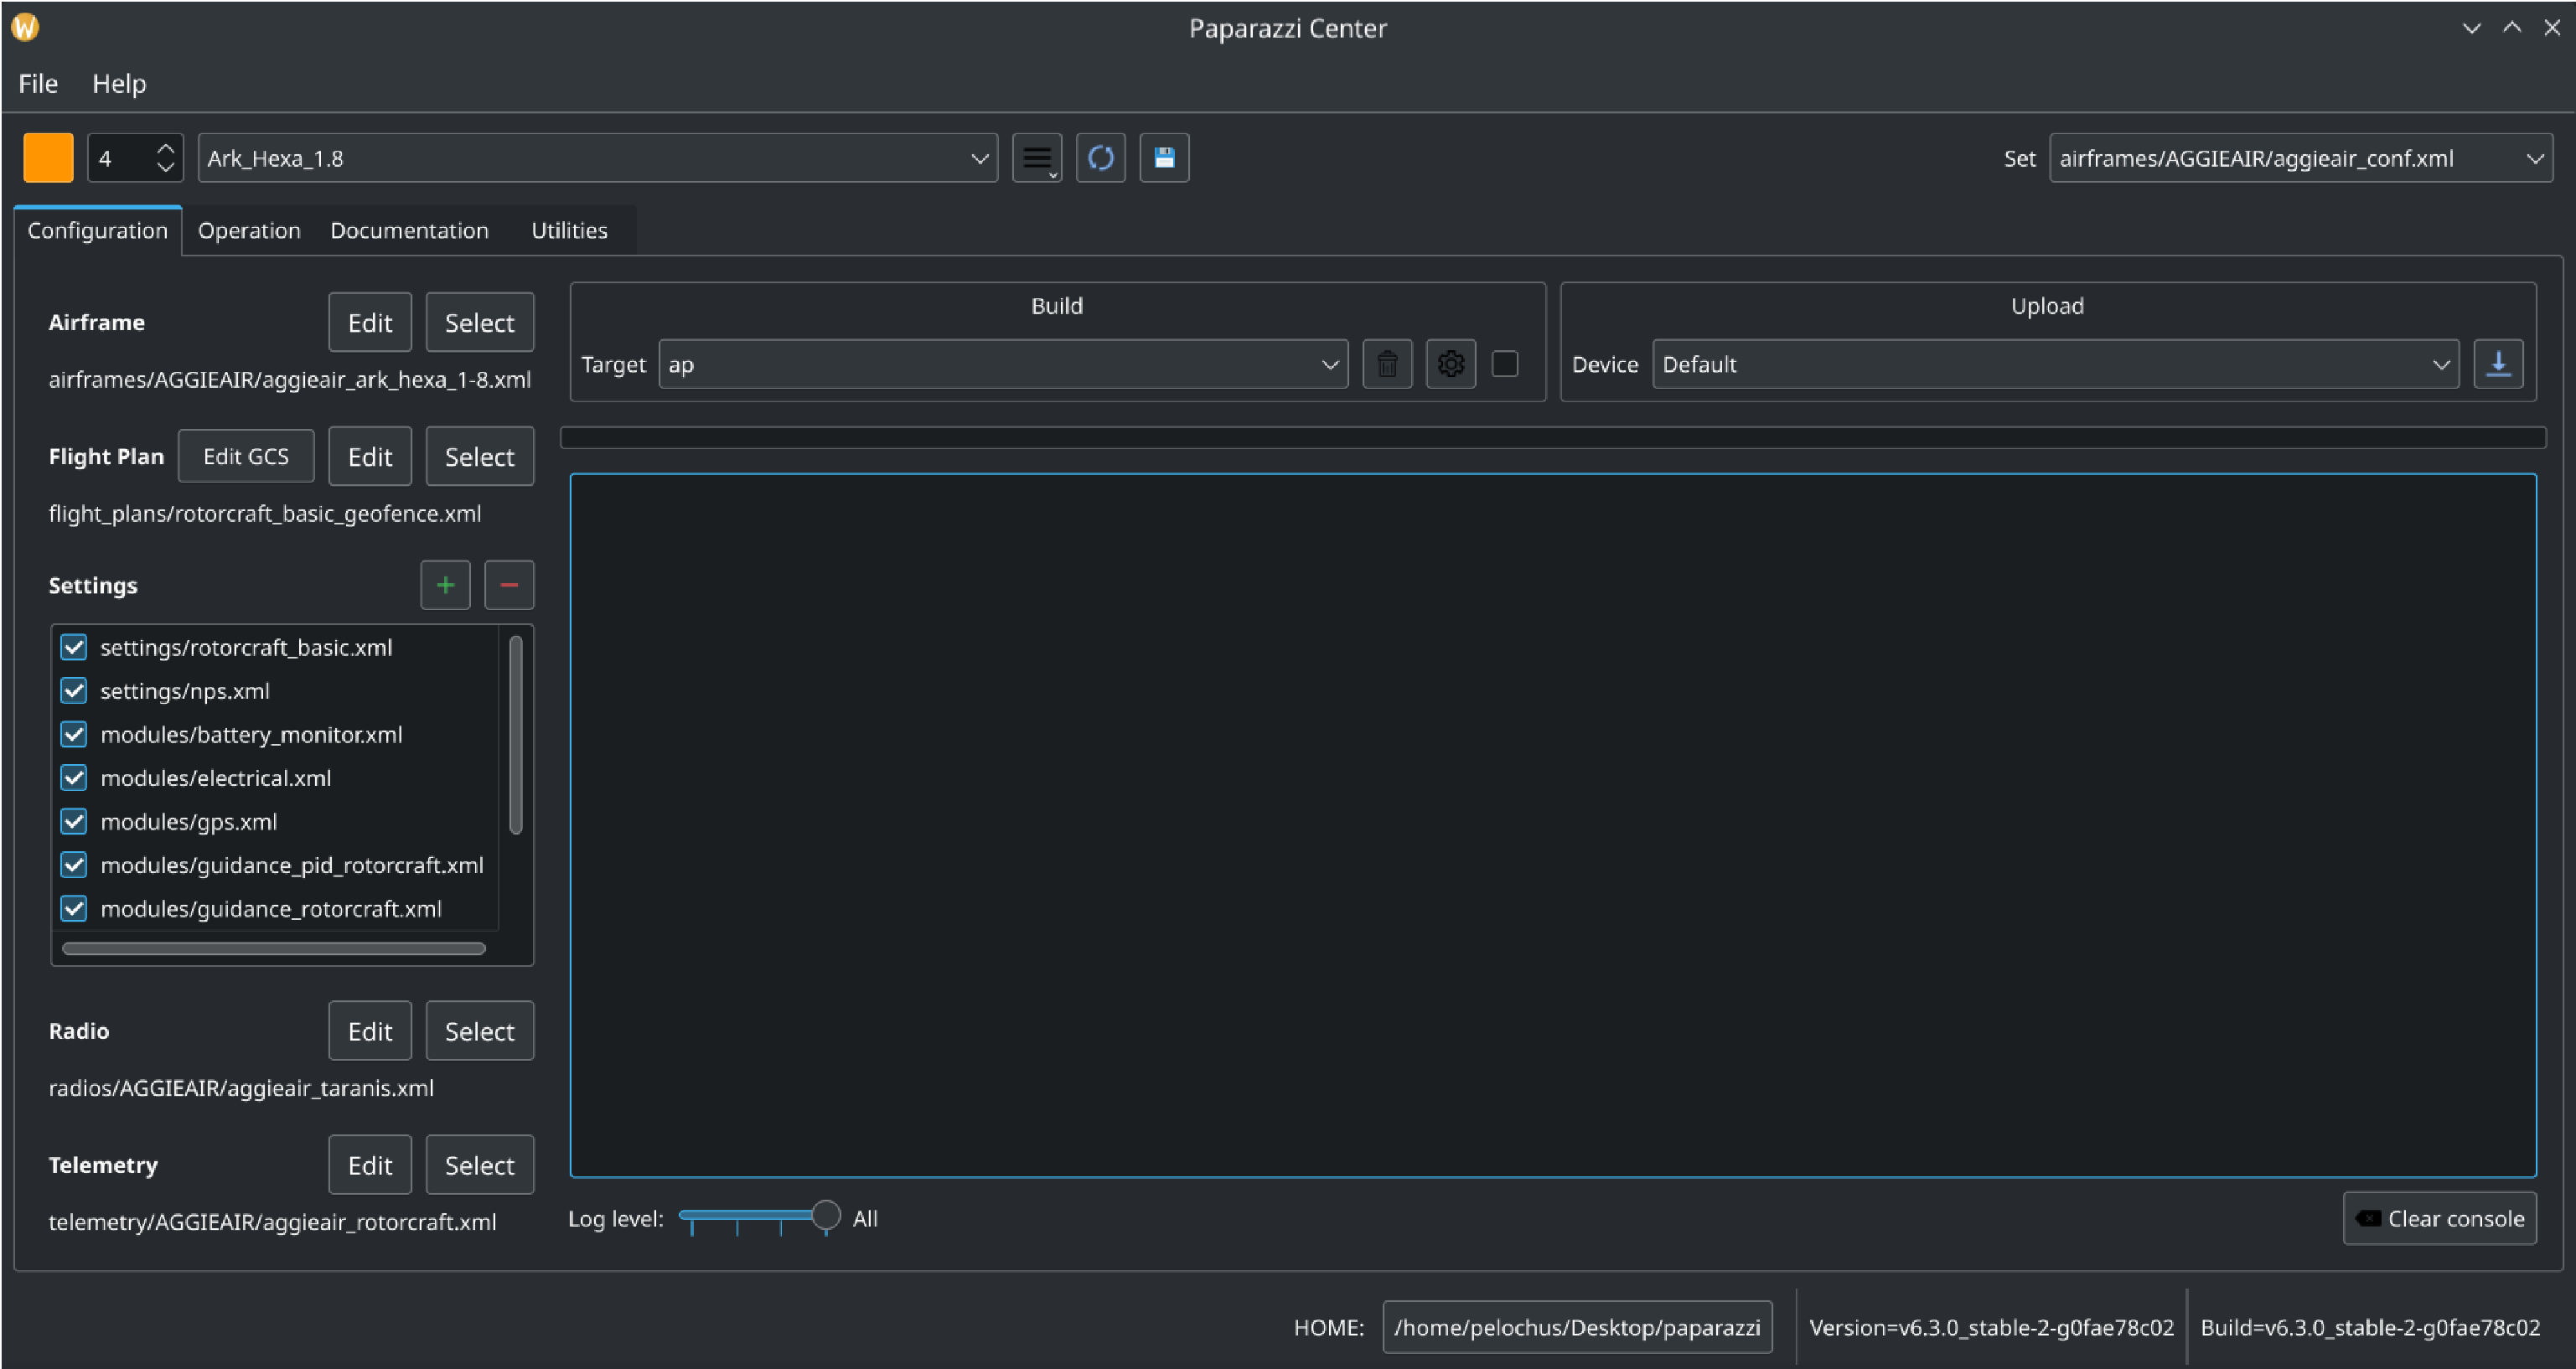
\includegraphics[width=0.92\textwidth]{img/fig/fig2.5-paparazzi-center.png}
    \caption{Captura de Paparazzi Center bajo Debian 12 con KDE}
    \label{fig:paparazzi-center}
\end{figure}

Desde Paparazzi Center se puede realizar simulaciones, planes de vuelo, observar mensajes de la consola, 
seleccionar el UAV deseado y un largo etcétera de posibilidades.
Se utilizará principalmente los paneles de operación de vuelo, simulación de vuelo, ajustes y consola para depuración.

%%%%%%%%%%%%%%%%%%%%%%%%%%%%%%%%%%%%%%%%%%%%%%%%%%%%%%%%%%%%%%%%%%%%%%%%%%%%%%%%%%%%%%%%%%%%%%%%%%%%%%%%%%%%%%%%%
%%%%%%%%%%%%%%%%%%%%%%%%%%%%%%%%%%%%%%%%%%%%%%%%%%%%%%%%%%%%%%%%%%%%%%%%%%%%%%%%%%%%%%%%%%%%%%%%%%%%%%%%%%%%%%%%%
%%%%%%%%%%%%%%%%%%%%%%%%%%%%%%%%%%%%%%%%%%%%%%%%%%%%%%%%%%%%%%%%%%%%%%%%%%%%%%%%%%%%%%%%%%%%%%%%%%%%%%%%%%%%%%%%%

\subsection{Simulaciones en Paparazzi Center}

Siguiendo la documentación de Paparazzi  podemos realizar la primera simulación \cite{paparazzi_first_simulation}. 
Seguir los pasos resulta en la apertura de Paparazzi GCS.

\begin{figure}[h]
    \centering
    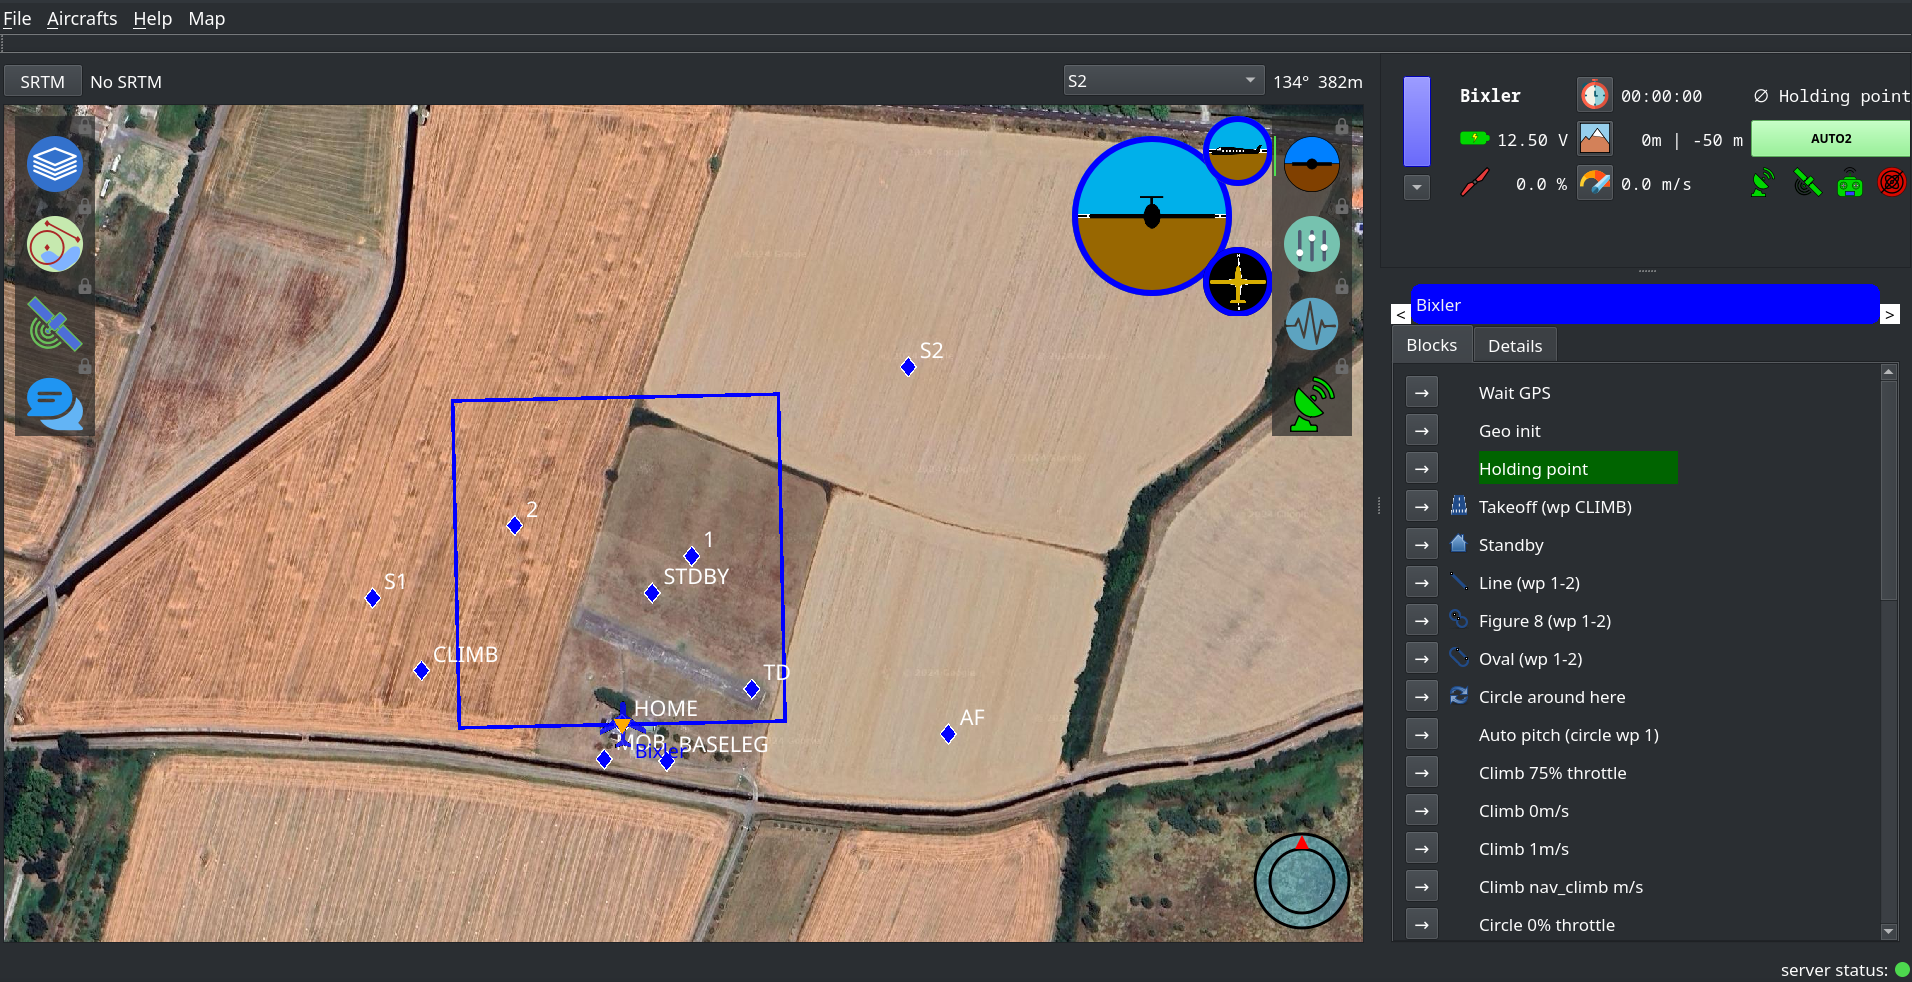
\includegraphics[width=0.9\textwidth]{img/fig/fig2.6-paparazzi-gcs-first-sim.png}
    \caption{Paparazzi GCS ejecutando la simulación por defecto}
    \label{fig:paparazzi-first-simulation}
\end{figure}

Desde Paparazzi GCS tenemos un sinfín de posibilidades más que desde Crazyflie Client. Cabe destacar, por ejemplo,
la capacidad realizar simulaciones en una zona del planeta cualquiera. Esto se puede aplicar a las misiones de 
vuelo reales, es decir, mediante GPS indicar en que zona estamos volando. 

Por otro lado, tenemos la capacidad de observar una gran cantidad de variables, incluso personalizar cuales 
queremos ver y cuales no, controles y órdenes de todo tipo, capacidad para elegir \textit{waypoints} etc...

%%%%%%%%%%%%%%%%%%%%%%%%%%%%%%%%%%%%%%%%%%%%%%%%%%%%%%%%%%%%%%%%%%%%%%%%%%%%%%%%%%%%%%%%%%%%%%%%%%%%%%%%%%%%%%%%%
%%%%%%%%%%%%%%%%%%%%%%%%%%%%%%%%%%%%%%%%%%%%%%%%%%%%%%%%%%%%%%%%%%%%%%%%%%%%%%%%%%%%%%%%%%%%%%%%%%%%%%%%%%%%%%%%%
%%%%%%%%%%%%%%%%%%%%%%%%%%%%%%%%%%%%%%%%%%%%%%%%%%%%%%%%%%%%%%%%%%%%%%%%%%%%%%%%%%%%%%%%%%%%%%%%%%%%%%%%%%%%%%%%%

\subsection{Firmware de Paparazzi para Crazyflie 2.1}

\begin{figure}[h]
    \centering
    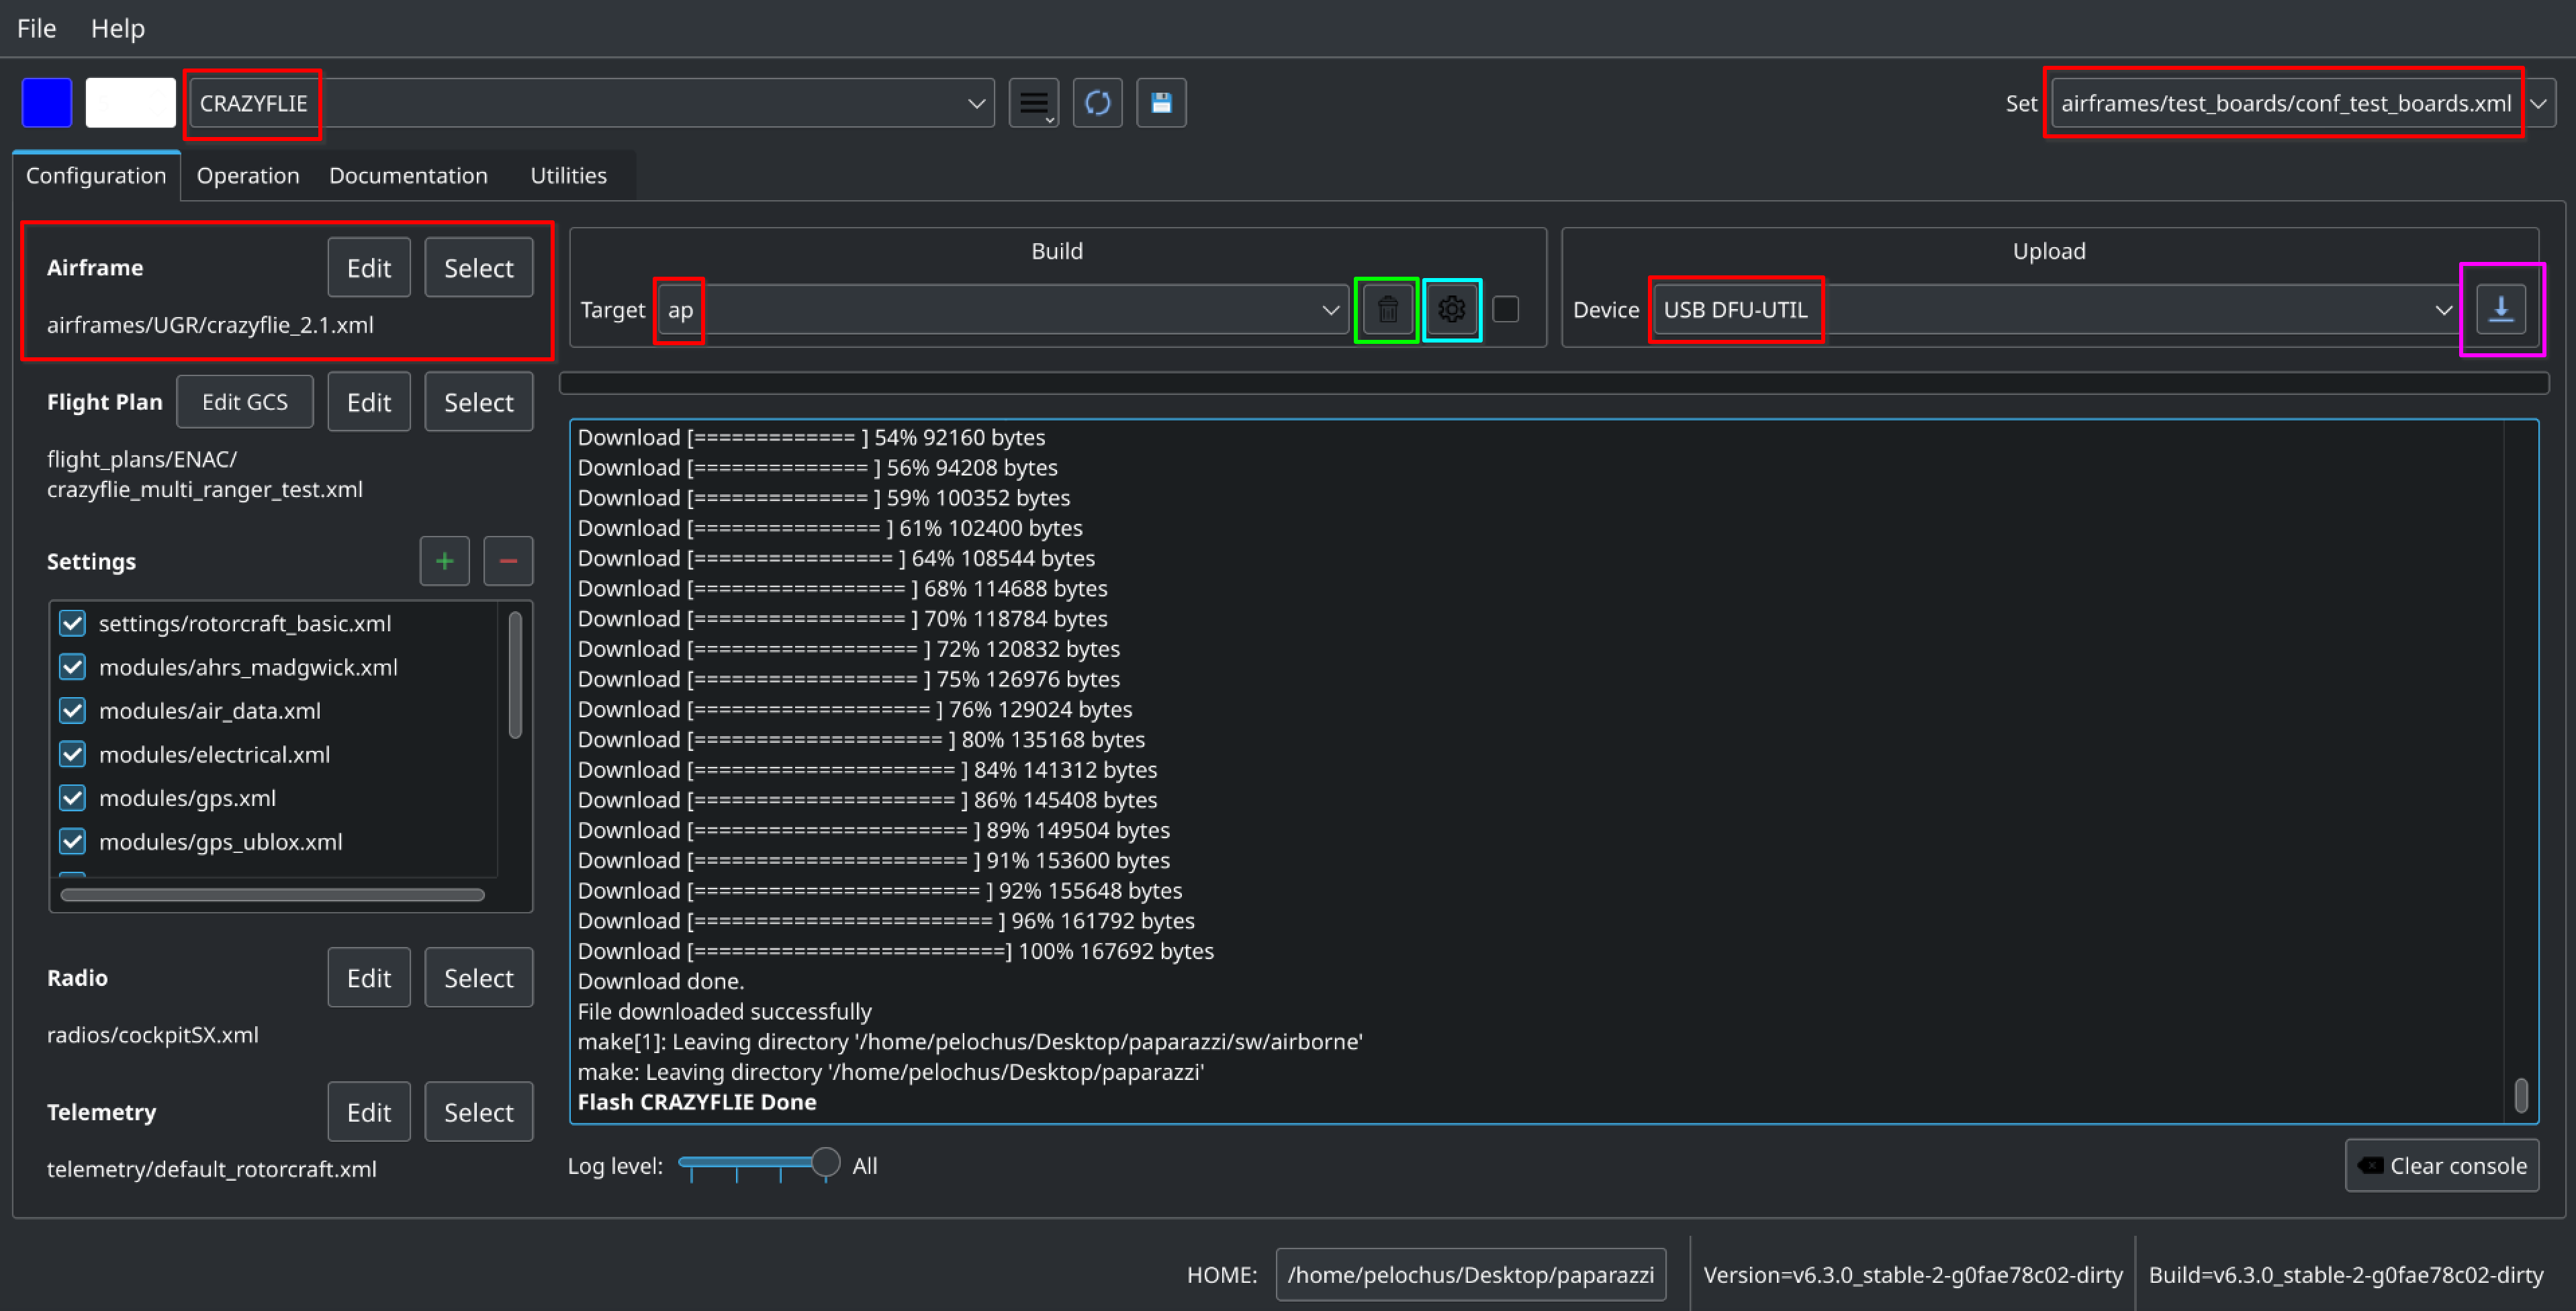
\includegraphics[width=0.99\textwidth]{img/fig/fig2.7-flash-paparazzi.png}
    \caption{Ajustes para cargar el firmware de Crazyflie en Paparazzi}
    \label{fig:upload-firmware-crazyflie}
\end{figure}

Se seguirá la guía oficial para cargar el firmware \cite{paparazzi_crazyflie}. Previamente, es necesario utilizar una versión previa del firmware oficial para conseguir compatibilidad con el firmware de Paparazzi \cite{crazyflie-firmware-fix}.
Este procedimiento consiste en los siguientes pasos:

\begin{enumerate}
    \item Se instalan las dependencias necesarias. Se encuentran el repositorio de este TFG \cite{bt-crazyflies}.
    Para un lector que no vaya a hacer pruebas, se recomienda leer el \autoref{appendix:crazyflie_dependencies}, que contiene más detalles.

    \item Se mantiene presionado el botón de encendido del Crazyflie mientras se conecta por USB.
    Esto permite entrar en el modo DFU, que permite cambiar el firmware.

    \item Desde Paparazzi se carga el firmware acorde con la \autoref{fig:upload-firmware-crazyflie}:

    \begin{enumerate}
        \item Se ajustan los parámetros que estan en \textcolor{red}{rojo} de la misma forma.
        
        \item Se pulsa el botón resaltado en \textcolor{Green3}{verde}, para limpiar archivos, análogo de Paparazzi a hacer un \textit{make clean} al compilar un ejecutable.
        
        \item Se pulsa el botón resaltado en \textcolor{cyan}{cyan}, para autocompilar el firmware. De nuevo, podemos hacer analogía con \textit{make}.

        \item Se pulsa el botón en \textcolor{violet}{morado} para cargar finalmente el firmware en el Crazyflie. Esto no debería fallar si se han seguido correctamente los pasos para instalar dependencias.
    \end{enumerate}
\end{enumerate}

Por último, se debe probar que Paparazzi funciona en el Crazyflie. 
Se probará la conexión mediante Crazyradio. Se siguen los siguientes pasos:

\begin{enumerate}
    \item Para empezar, es necesario haber instalado las dependencias.
    Se incluyen en el previamente mencionado \autoref{appendix:crazyflie_dependencies}.

    \item Siguiendo la \autoref{fig:crazyradio-paparazzi-center} 
    podemos conectar un Crazyflie a Paparazzi Center usando la Crazyradio.
    Se siguen los siguientes pasos:

    \begin{enumerate}
        \item Se añade uso del Crazyradio 2.0 mediante el menú \textit{Add Tool - Crazyradio/IvyBridge}.
        Esto añade la configuración marcada en \textcolor{red}{rojo}.
        
        \item Similarmente, desde el menú \textit{Add Tool - Messages} se añade la configuración marcada en \textcolor{Green3}{verde}. 
        Además aparece la ventana señalada en \textcolor{violet}{morado} tras seleccionar el módulo, que muestra la recepción y envío de datos.
    \end{enumerate}
\end{enumerate}

\begin{figure}[!h]
    \centering
    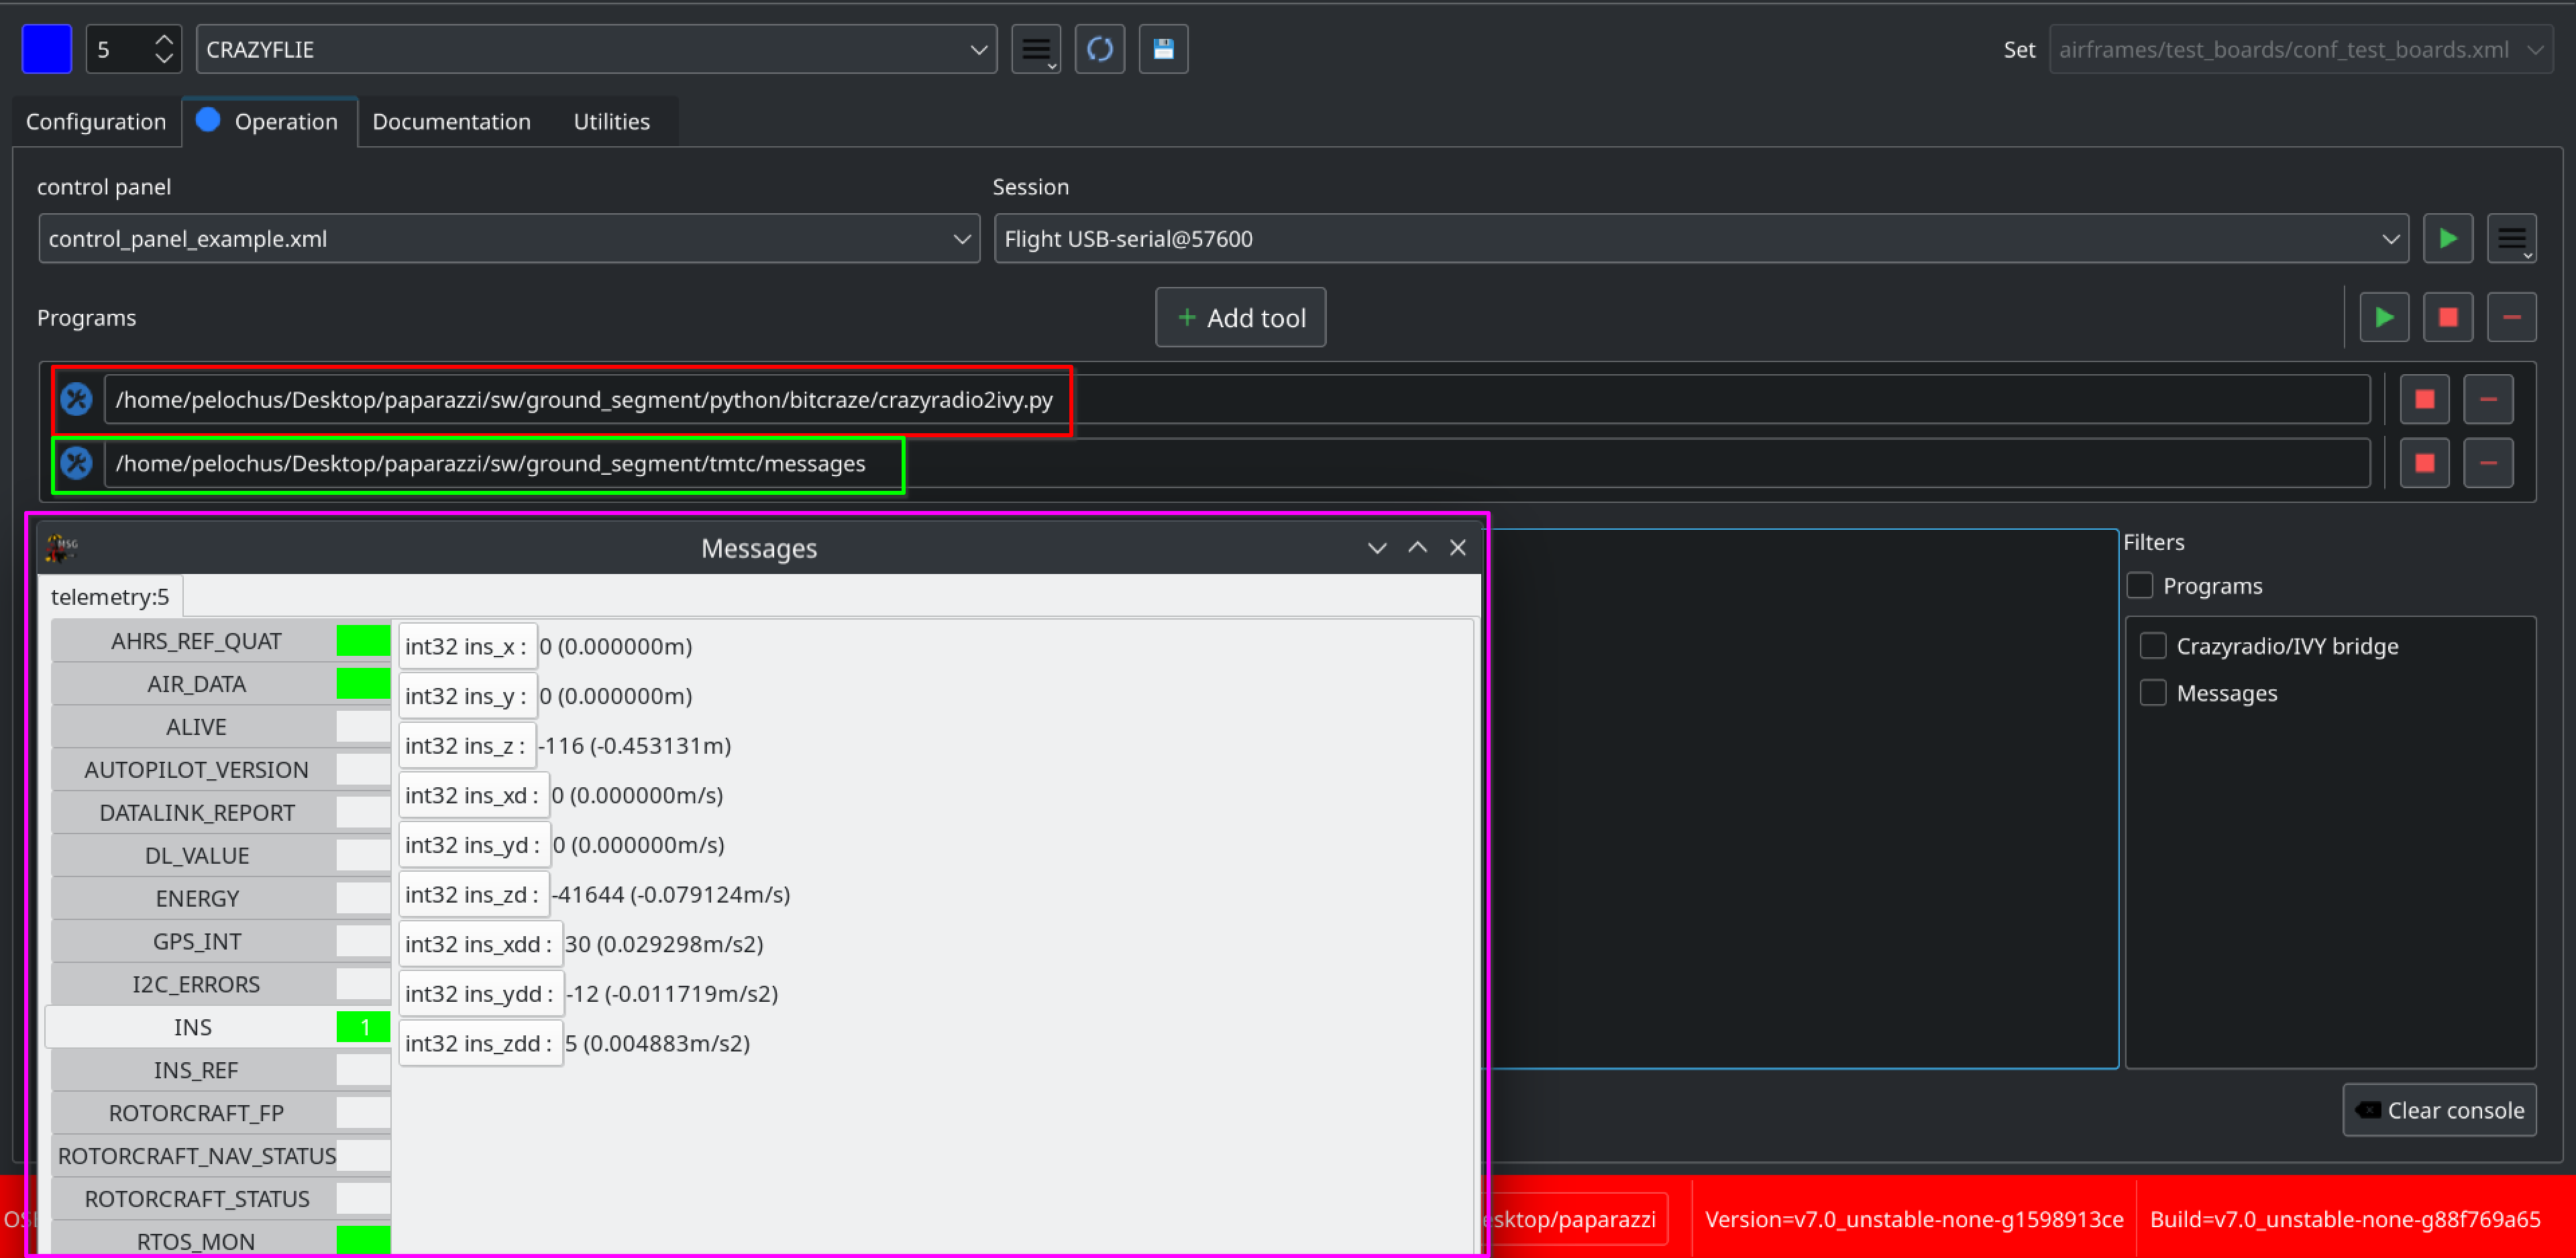
\includegraphics[width=0.85\textwidth]{img/fig/fig2.8-radio-connection.png}
    \caption{Conexión del Crazyradio al Crazyflie mediante Paparazzi}
    \label{fig:crazyradio-paparazzi-center}
\end{figure}

%%%%%%%%%%%%%%%%%%%%%%%%%%%%%%%%%%%%%%%%%%%%%%%%%%%%%%%%%%%%%%%%%%%%%%%%%%%%%%%%%%%%%%%%%%%%%%%%%%%%%%%%%%%%%%%%%
%%%%%%%%%%%%%%%%%%%%%%%%%%%%%%%%%%%%%%%%%%%%%%%%%%%%%%%%%%%%%%%%%%%%%%%%%%%%%%%%%%%%%%%%%%%%%%%%%%%%%%%%%%%%%%%%%
%%%%%%%%%%%%%%%%%%%%%%%%%%%%%%%%%%%%%%%%%%%%%%%%%%%%%%%%%%%%%%%%%%%%%%%%%%%%%%%%%%%%%%%%%%%%%%%%%%%%%%%%%%%%%%%%%

\section{Desarrollo básico en Paparazzi}

Es importante entender como se desarrolla módulos de control en Paparazzi. 
Los módulos se ocupan de controlar el UAV correspondiente de la forma más génerica posible,
permitiendo que varios UAVs distintos puedan utilizar un mismo módulo. 
Además, permiten adaptar la interfaz del GCS para, por ejemplo, colocar un deslizador que permita cambiar el control de una variable como la velocidad de un UAV.

En esta sección se desarrollará un pequeño módulo de ejemplo según la guía oficial \cite{modules-paparazzi}
de Paparazzi, así se puede entender mejor como se desarrollará este TFG.

%%%%%%%%%%%%%%%%%%%%%%%%%%%%%%%%%%%%%%%%%%%%%%%%%%%%%%%%%%%%%%%%%%%%%%%%%%%%%%%%%%%%%%%%%%%%%%%%%%%%%%%%%%%%%%%%%
%%%%%%%%%%%%%%%%%%%%%%%%%%%%%%%%%%%%%%%%%%%%%%%%%%%%%%%%%%%%%%%%%%%%%%%%%%%%%%%%%%%%%%%%%%%%%%%%%%%%%%%%%%%%%%%%%
%%%%%%%%%%%%%%%%%%%%%%%%%%%%%%%%%%%%%%%%%%%%%%%%%%%%%%%%%%%%%%%%%%%%%%%%%%%%%%%%%%%%%%%%%%%%%%%%%%%%%%%%%%%%%%%%%

\subsection{Desarrollo de módulos de control}

Paparazzi define los módulos en XML. 
Este formato permite una estructura clara y modular para implementación de módulos pero no permite el desarrollo de código. 
Para solucionar esto, el código de los módulos se implementa en el lenguaje C, 
en el cual se puede implementar algoritmos de control o manejar datos de, por ejemplo, sensores. Estos XML se encuentran en \texttt{./conf/modules/}.

La principal utilidad de los módulos aparece al compilar un firmware, donde se indica que módulos se usarán para el control del dispositivo. 
Por ejemplo, un dron con GPS y acelerómetro podrá incluir el módulo de control GPS de Paparazzi y de uso del acelerómetro. 
También existen módulos génericos, que permiten para un tipo de dispositivo, incluir los módulos básicos. 
Para un rotorcraft, será por lo general módulos de control de 4 motores, IMU 
(\textit{Inertial Measurement Unit} que incluye acelerómetro y giroscopos), control por radio etc...

Aquí vemos el módulo de demostración de Paparazzi.

\begin{lstlisting}[style=CodigoXML]
<!DOCTYPE module SYSTEM "module.dtd">

<module name="demo_module">
  <doc>
    <description>Demo module</description>
  </doc>
  <header>
    <file name="demo_module.h"/>
  </header>
  <init fun="init_demo()"/>
  <periodic fun="periodic_1Hz_demo()" freq="1." start="start_demo()" stop="stop_demo()" autorun="TRUE"/>
  <periodic fun="periodic_10Hz_demo()" period="0.1" start="start_demo()" stop="stop_demo()" autorun="FALSE"/>
  <makefile>
    <raw>
#Example of RAW makefile part
    </raw>
    <define name="DEMO_MODULE_LED" value="2"/>
    <file name="demo_module.c"/>
  </makefile>
  <makefile target="demo">
    <define name="SOME_FLAG"/>
    <configure name="SOME_DEFINE" value="bla"/>
  </makefile>
</module>
\end{lstlisting}

Por otro lado, es importante entender que la programación de los módulos esta en C. 
Estos archivos, por su parte, se encuentran en 
\texttt{./sw/airborne/modules/}
Por ejemplo, veamos el código C para el módulo de demostración:

\begin{lstlisting}[style=CodigoC]
#include "demo_module.h"
#include "led.h"

void init_demo(void)
{
  // this part is already done by led_init in fact
  LED_INIT(DEMO_MODULE_LED);
  LED_OFF(DEMO_MODULE_LED);
}

void periodic_1Hz_demo(void)
{
  LED_TOGGLE(DEMO_MODULE_LED);
}

void periodic_10Hz_demo(void)
{
  LED_TOGGLE(DEMO_MODULE_LED);
}

void start_demo(void)
{
  LED_ON(DEMO_MODULE_LED);
}

void stop_demo(void)
{
  LED_OFF(DEMO_MODULE_LED);
}
\end{lstlisting}

En conjunto, ambos archivos previos mostrados permiten generar automáticamente el encendido y apagado de un LED de forma periódica en un sistema usando el firmware de Paparazzi. 
Como bien se ha explicado antes, se puede diferenciar de forma que el archivo C permite generar la lógica mínima de control (en este caso, de los LEDs) 
y el archivo XML añade documentación, ajustes para compilación, frecuencia o periodicidad de cada función... entre otras funciones.

La razón del uso de archivos de XML, además de modularidad y claridad, es debido al uso extendido de ChibiOS en Paparazzi \cite{chibios-paparazzi}, 
un sistema operativo de tiempo real que se ocupa de ejecutar las funciones de forma periódica como bien permite definir el XML, 
utilizando, como es propio de un sistema RT, diversos hilos de ejecución. 

Existe la posibilidad de no usar ChibiOS y utilizar un programa en bucle, no obstante, no es el comportamiento más usado, ni generalmente preferible. 
La plataforma \textbf{Crazyflie 2.1 en Paparazzi utiliza ChibiOS}. 

Finalmente, hay que añadir al archivo de configuración del firmware del Crazyflie en Paparazzi este pequeño trozo de código para que, en este caso el Crazyflie, pueda ejecutar el módulo de demostración:

\begin{lstlisting}[style=CodigoXML]
<module name="demo_module"/>
\end{lstlisting}

En general, se puede resumir la estructura de los módulos y como se ubican en Paparazzi con el siguiente diagrama:

\begin{figure}[h]
    \centering
    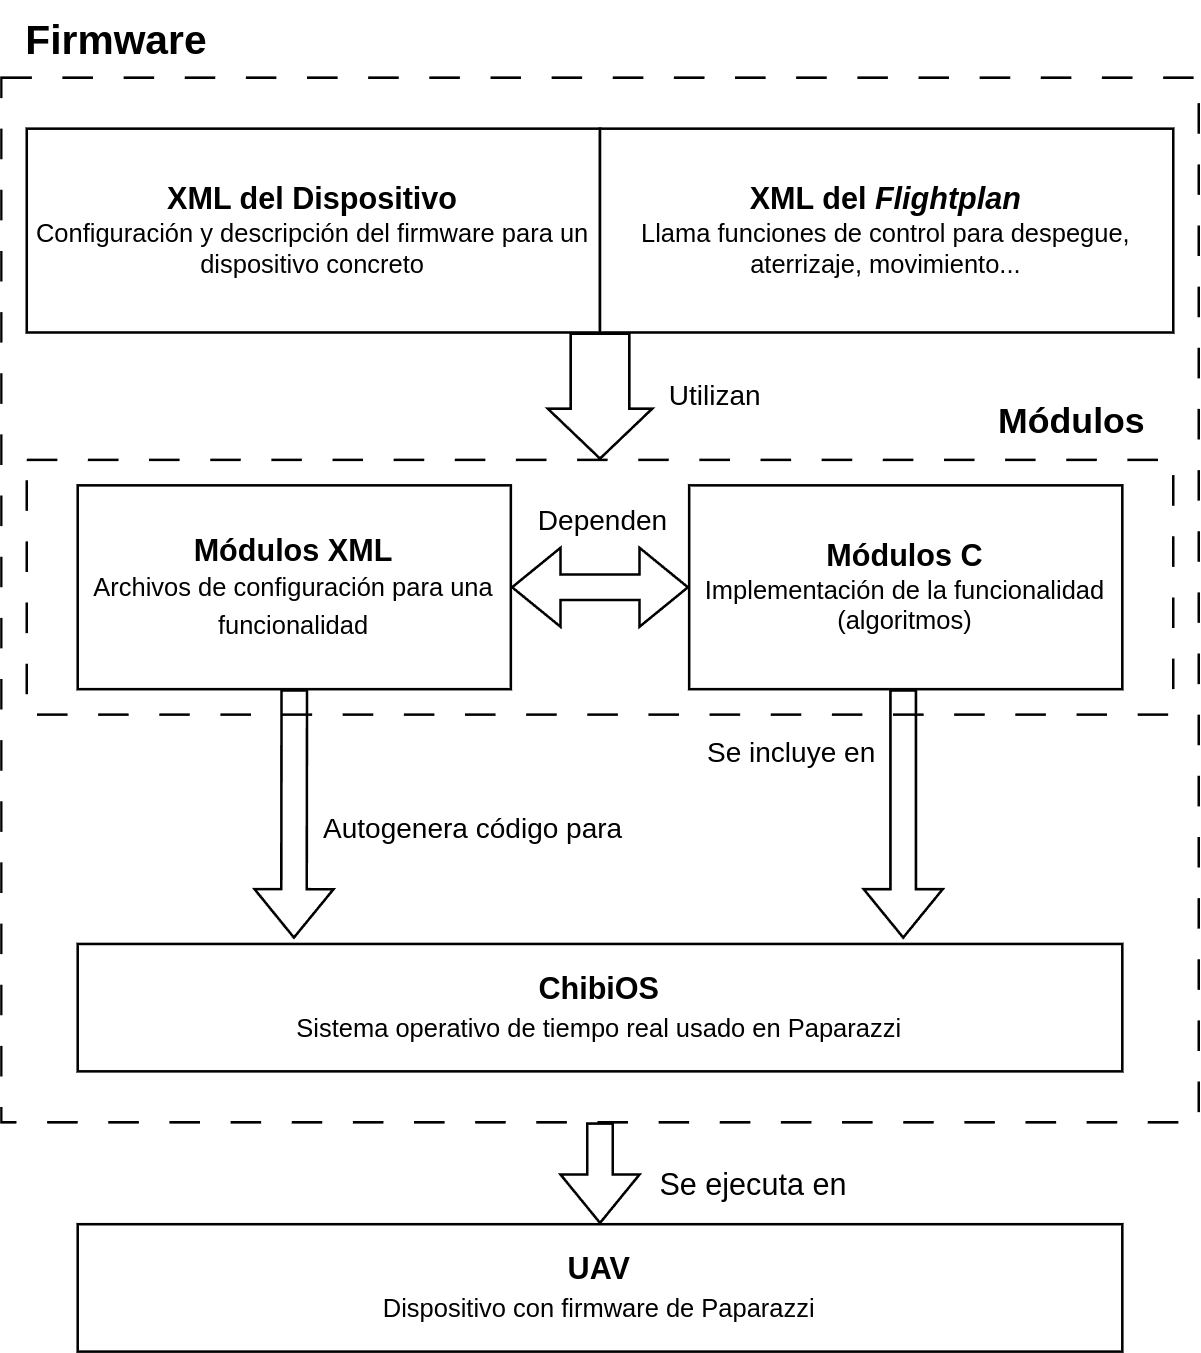
\includegraphics[width=0.72\textwidth]{img/fig/fig2.9-firmware-paparazzi.png}
    \caption{Estructura del firmware de Paparazzi}
    \label{fig:firmware-paparazzi}
\end{figure}

%%%%%%%%%%%%%%%%%%%%%%%%%%%%%%%%%%%%%%%%%%%%%%%%%%%%%%%%%%%%%%%%%%%%%%%%%%%%%%%%%%%%%%%%%%%%%%%%%%%%%%%%%%%%%%%%%
%%%%%%%%%%%%%%%%%%%%%%%%%%%%%%%%%%%%%%%%%%%%%%%%%%%%%%%%%%%%%%%%%%%%%%%%%%%%%%%%%%%%%%%%%%%%%%%%%%%%%%%%%%%%%%%%%
%%%%%%%%%%%%%%%%%%%%%%%%%%%%%%%%%%%%%%%%%%%%%%%%%%%%%%%%%%%%%%%%%%%%%%%%%%%%%%%%%%%%%%%%%%%%%%%%%%%%%%%%%%%%%%%%%

\subsection{Uso de módulos en una simulación}

En esta sección se verá en ejecución el módulo de demostración de la sección anterior. 
Los módulos permiten añadir comportamientos y funcionalidades extra a los dispositivos con Paparazzi. 
Normalmente, este comportamiento se puede observar desde Paparazzi GCS. 
En la siguiente figura podemos ver el módulo de demostración en Paparazzi GCS.

\begin{figure}[h]
    \centering
    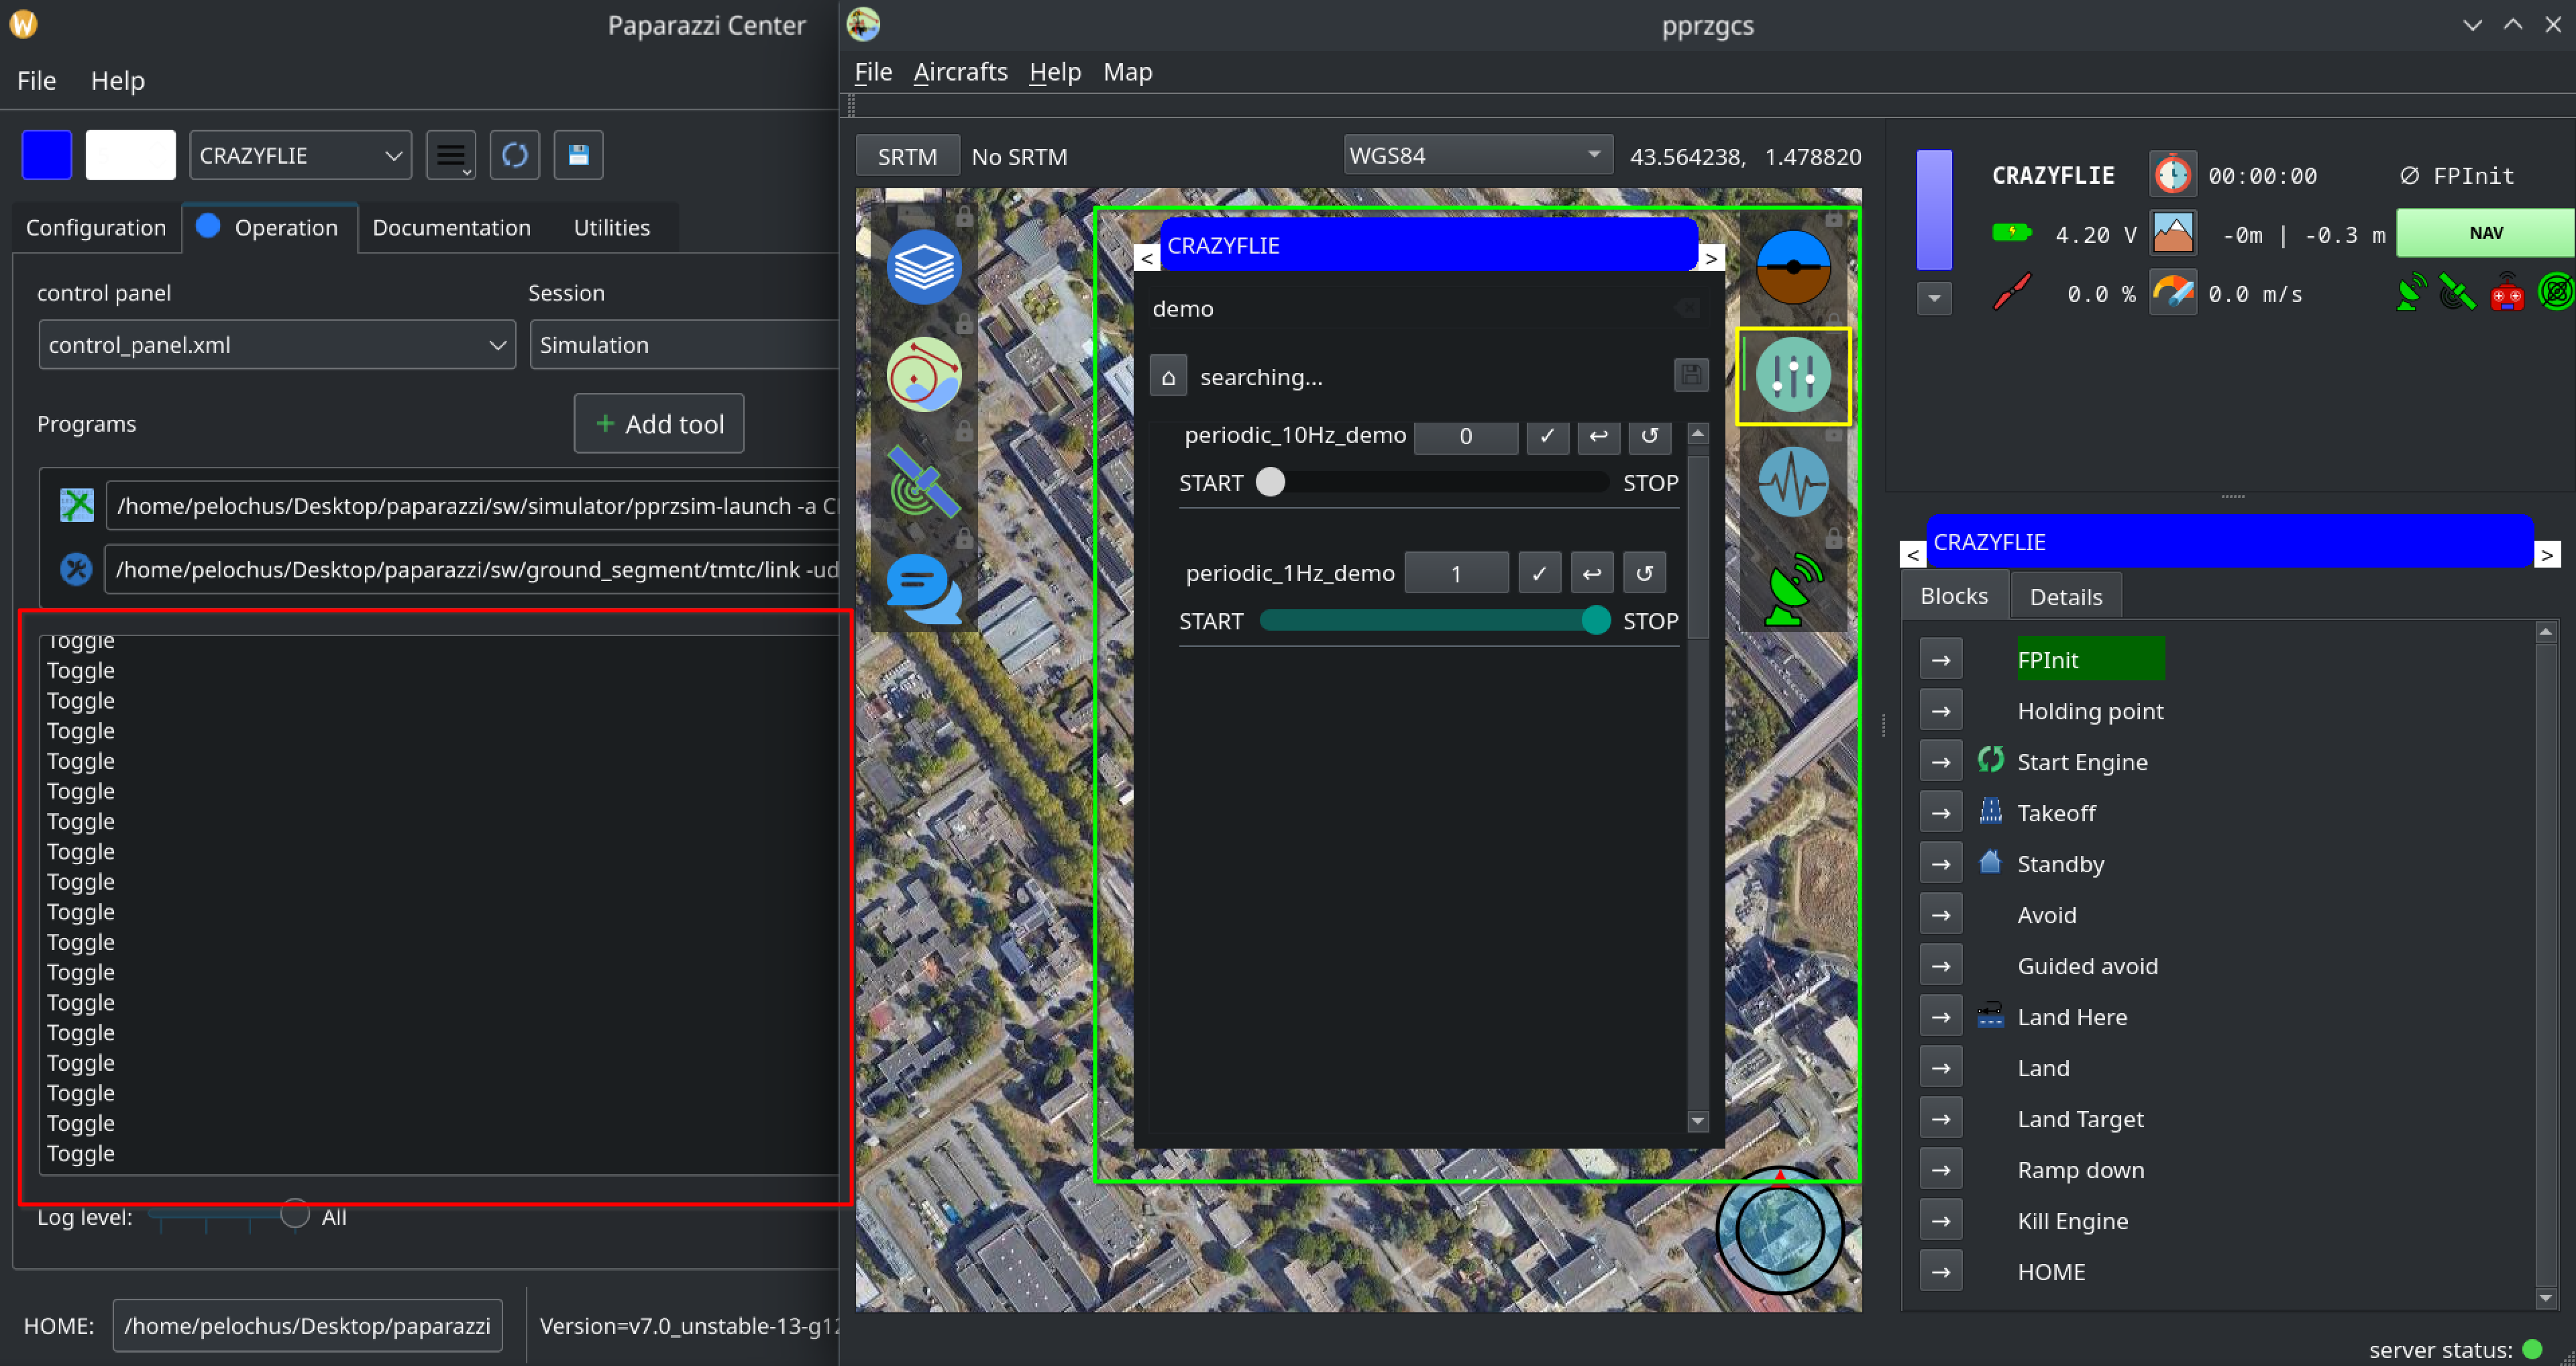
\includegraphics[width=0.99\textwidth]{img/fig/fig2.10-demo-module.png}
    \caption{Módulo de demostración en Paparazzi}
    \label{fig:demo-module-paparazzi}
\end{figure}

Si nos fijamos en la figura, podemos dividir por las siguientes partes:

\begin{enumerate}
    \item Se asume que se parte de una simulación, con Paparazzi GCS ya ejecutándose

    \item Desde el menú rodeado en color \textcolor{Green3}{verde}, podemos ajustar parámetros del módulo. 
    Para mostrar este menú se presiona el botón rodeado en \textcolor{Gold3}{amarillo}.
    
    \item Por último, podemos ver los resultados en la terminal rodeada en \textcolor{red}{rojo}.
    Al ser una simulación, simplemente se imprime por pantalla lo que se supone que se esta haciendo,
    en este caso cambiar el LED de estado cada segundo.
\end{enumerate}

Con los Crazyflies montados, funcionales con Paparazzi y entendido el funcionamiento básico de este, 
el siguiente capítulo consistirá en empezar el desarrollo para este dron en el marco de Paparazzi.